\chapter{Projekt systemu}
W tym rozdziale zostanie opisany projekt systemu oraz przedstawiona analiza wymagań pod kątem przypadków użycia. Następnie każdy przypadek użycia zostanie omówiony, a jego działanie zilustrowane za pomocą makiet aplikacji. Pierwszym podpunktem będzie identyfikacja aktorów.

\section{Identyfikacja aktorów}
Biorąc pod uwagę założenia opisane w poprzednich podrozdziałach, zaprojektowany został diagram przypadków użycia aplikacji. Idnetyfikacja aktorów:
\begin{enumerate}
\item Użytkownik - ogólny użytkownik systemu. Reprezentuje dowolną osobę korzystającą z serwisu, jego przypadki użycia będą dziedziczone przez pozostałych aktorów systemu.
\begin{figure}[H]
	\centering
		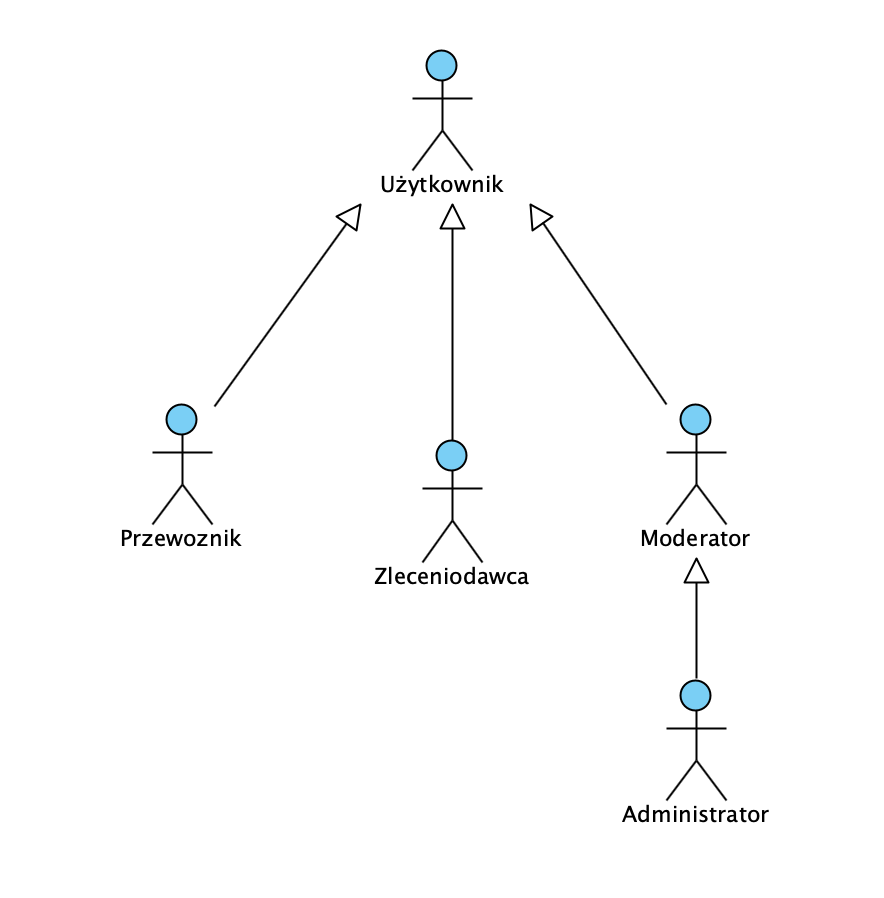
\includegraphics[width=0.6\linewidth]{rozdzial1/dziedziczenie.png}
	\caption{Graficzne ukazanie dziedziczenia możliwości aktorów}
	\label{Rys. fig:Graficzne ukazanie dziedziczenia możliwości aktorów}
\end{figure}
\item Przewoźnik - aktor odpowiedzialny za transport towarów. Może przeglądać dostępne zlecenia, dodawać ogłoszenia o planowanych trasach, komunikować się z autorami ogłoszeń, przyjmować zlecenia oraz oceniać i komentować kontrahentów.
\item Zleceniodawca - użytkownik systemu, który zleca transport towarów. Może dodawać nowe zlecenia transportowe, podobnie jak przewoźnik, może również przeglądać ogłoszenia przewoźników oraz komunikować się z autorami ogłoszeń.
\item Moderator - osoba odpowiedzialna za zarządzanie systemem. Moderator zatwierdza lub usuwa nowe ogłoszenia i zlecenia oraz blokuje konta użytkowników.
\item Administrator - użytkownik umiejscowiony najwyżej w hierarchii systemu. Może on wykonywać wszystko co moderator, lecz ma również możliwość dodawania nowych moderatorów lub usuwania obecnych.
\end{enumerate}

\section{Założenia wizualne}
Makieta aplikacji została wykonana w darmowym programie \texttt{Figma}, który pozwala na tworzenie interfejsu użytkownika i oferuje wiele funkcji ułatwiających pracę, takich jak utrzymanie spójności w rozmiarach czcionek, kolorach czy odstępach. Figma świetnie nadaje się także do tworzenia komponentów wielokrotnego użytku oraz ich wariantów. Komponenty te są również wykorzystywane w frameworku \texttt{Next.js}, dlatego uwzględnienie ich już na etapie projektowania ułatwia późniejszą implementację w kodzie.

Poniżej znajdują się założenia wizualne, które zostaną zastosowane podczas projektowania makiety aplikacji. Zdefinowane zostały wartości takie jak:
\begin{itemize}
    \item rozmiary czcionek dla odpowiednich elementów aplikacji,
    \item paleta kolorów,
    \item trzy warianty przycisków, główny, drugorzędny oraz trzeciorzędny,
    \item wygląd hiperłącz na stronie,
    \item przycisk do wybierania wersji językowej,
    \item warianty odstępów między elementami,
    \item pola tekstowe (ang. \texttt{inputs}) wraz ze swoim drugim wariantem,
    \item pola jednokrotnego wyboru
\end{itemize}
\begin{figure}[H]
	\centering
		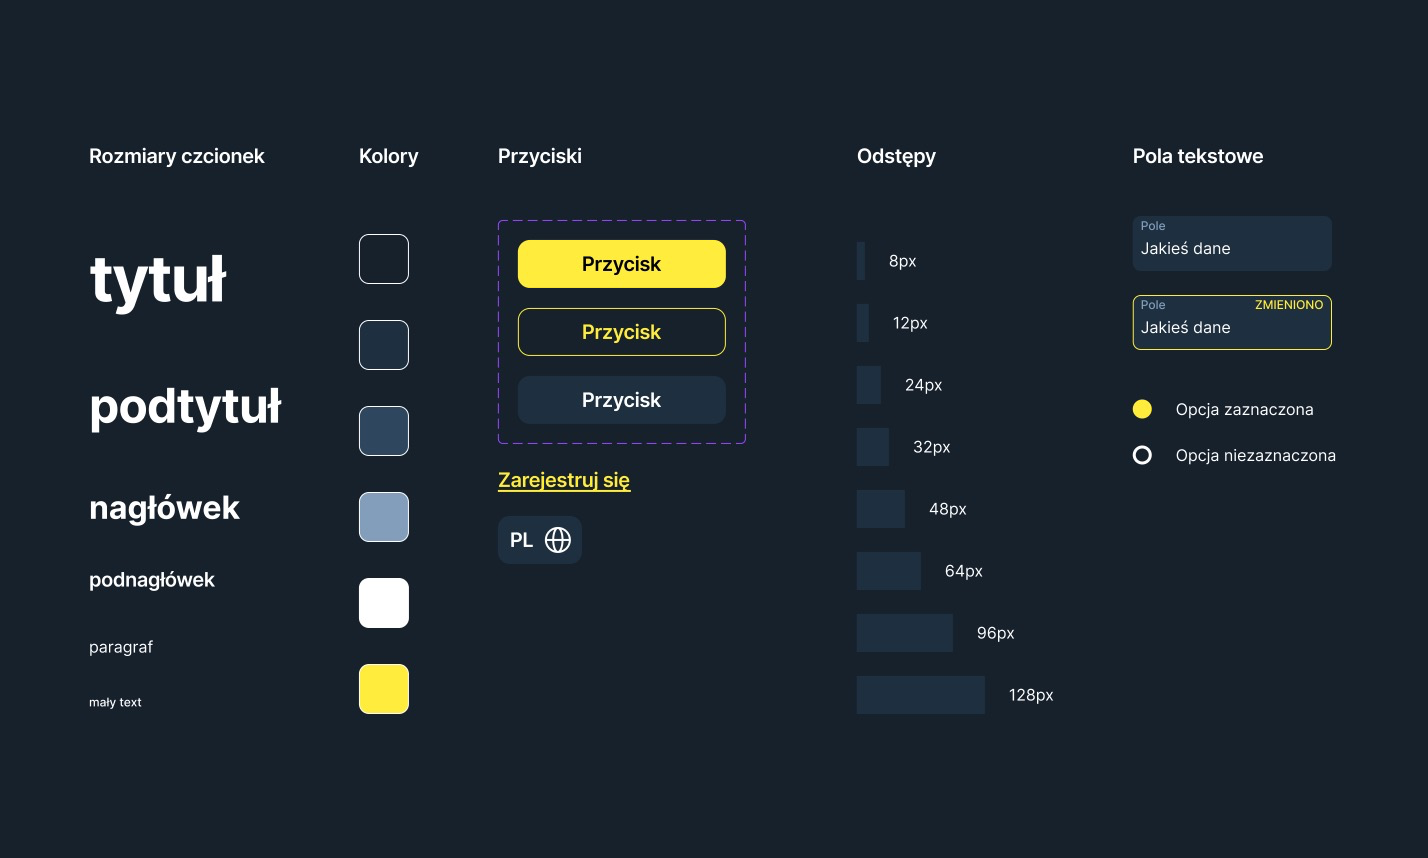
\includegraphics[width=0.7\linewidth]{rozdzial1/komponenty.png}
	\caption{Założenia co do aspektu wizualnego serwisu}
	\label{Rys. fig:Założenia wizualne serwisu}
\end{figure}

\section{Diagramy przypadków użycia}
W tej podrozdziale przedstawione zostaną diagramy przypadków użycia serwisu \texttt{CargoLink}, korzystając z definicji aktorów opisanych powyżej. Dodatkowo opisane i graficznie przedstawione zostaną wszystkie przypadki użycia użyte w diagramach.
\begin{figure}[H]
	\centering
		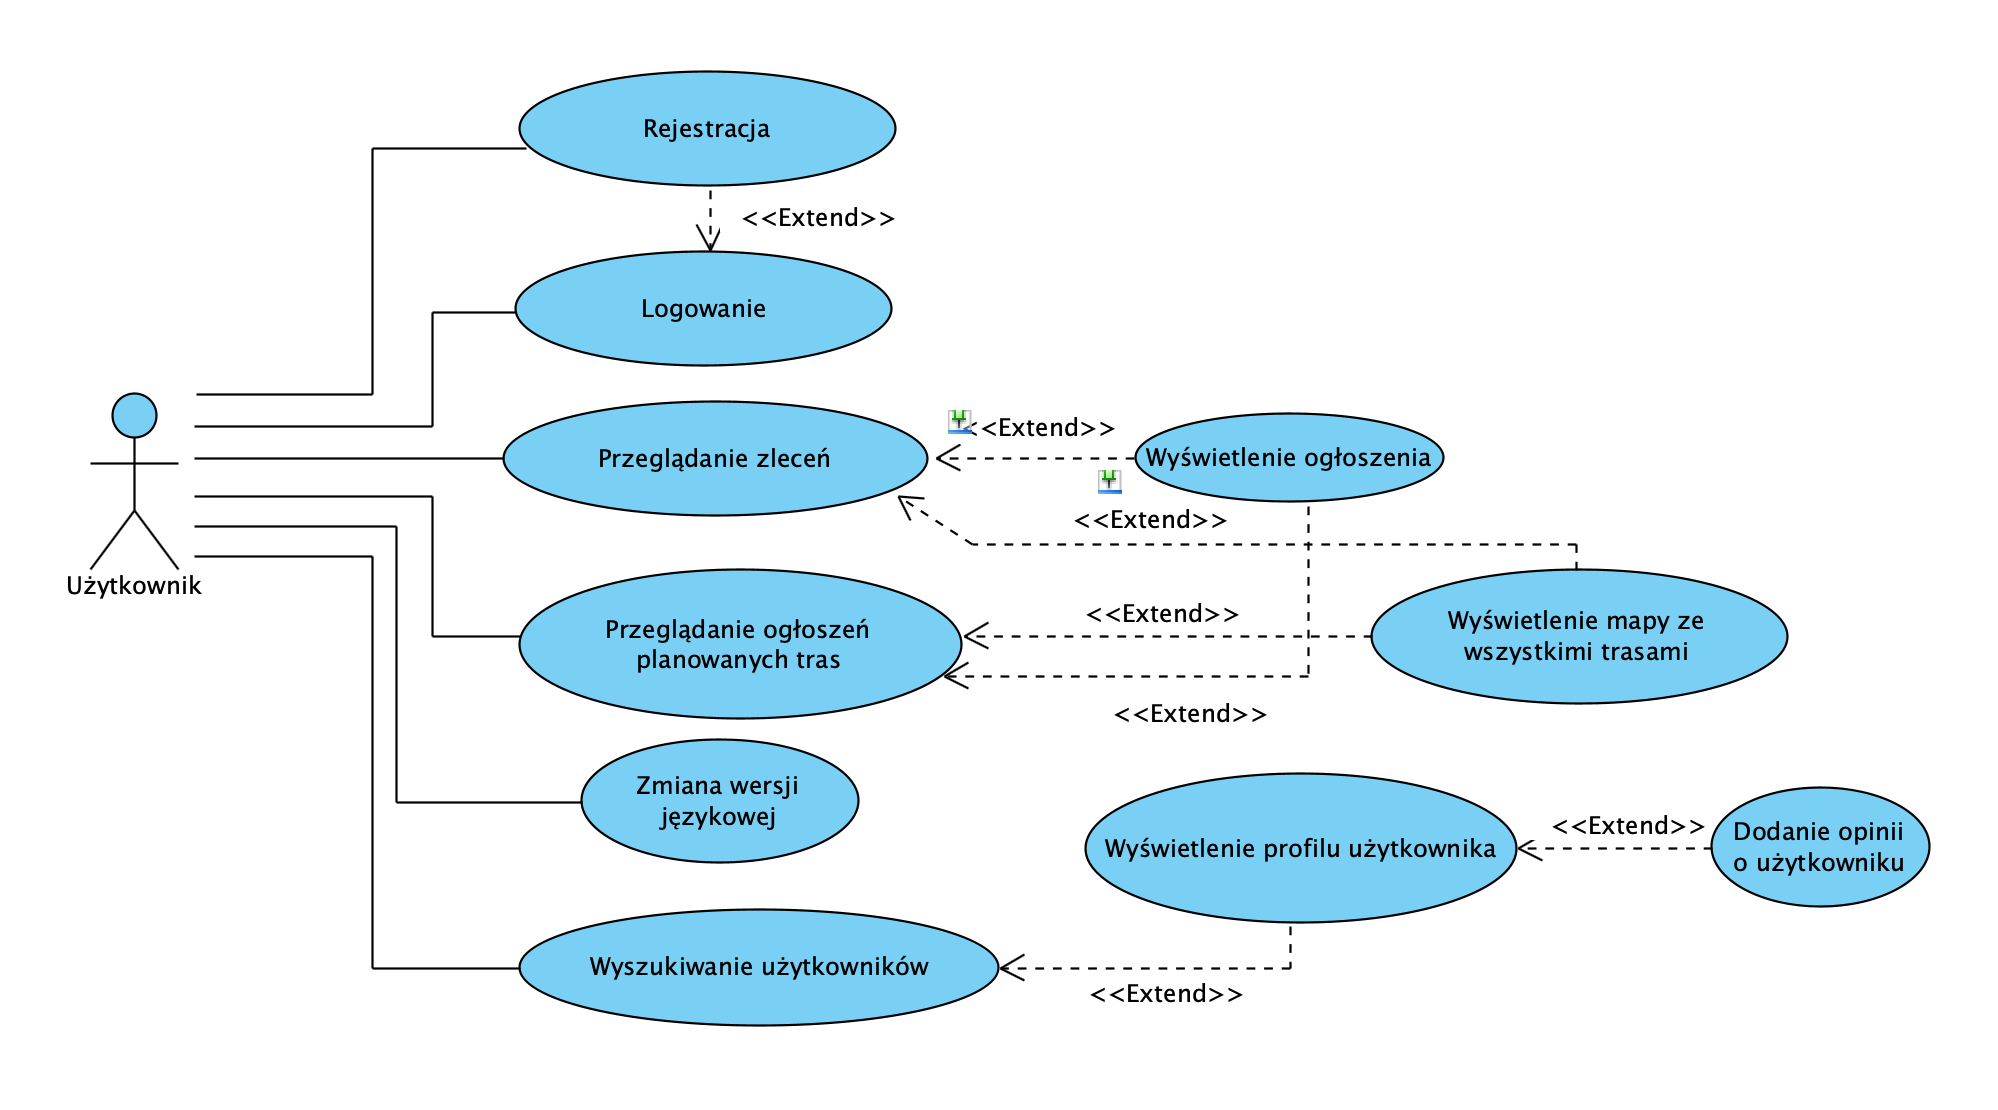
\includegraphics[width=\linewidth]{rozdzial1/PU_uzytkownik.png}
	\caption{Diagram przedstawiający przypadki użycia aktora Użytkownik}
	\label{Rys. fig:Diagram przedstawiający przypadki użycia aktora Użytkownik}
\end{figure}
Na powyższym obrazku przedstawiony został diagram przypadków użycia dla użytkownika. Będą one dziedziczone przez wszystkich pozostałych aktorów. \\

\textbf{Rejestracja} \\
Zdarzenie inicjujące: Kliknięcie przycisku \texttt{Nie masz konta? Zarejestruj się}. \\
Warunki początkowe: Użytkownik nie jest zalogowany. \\
Przebieg podstawowy realizacji przypadku użycia:
\begin{enumerate}
    \item Kliknięcie przycisku \texttt{Nie masz konta? Zarejestruj się} (Rys. \ref{fig:Formularz rejestracji - abc}.a);
    \item Wybór typu konta: zleceniodawca lub przewoźnik;
    \item Kliknięcie przycisku \texttt{dalej}; (Rys. \ref{fig:Formularz rejestracji - abc}.b)
    \item Wpisanie danych:
        \begin{itemize}
            \item imię,
            \item nazwisko,
            \item email (dwukrotnie w celu potwierdzenia),
            \item adres, miasto i ulica (w celu generowania umów między użytkownikami),
            \item numer telefonu,
            \item hasło (dwukrotnie w celu potwierdzenia)
        \end{itemize}
    \item Kliknięcie przycisku \texttt{Dalej}; (Rys. \ref{fig:Formularz rejestracji - abc}.c)
    \item System sprawdza w bazie danych czy istnieje już użytkownik o podanym emailu oraz sprawdza poprawność wprowadzonych danych;
    \item Wybór czy konto ma reprezentować przedsiębiorstwo (wymagane będzie podane pełnej nazwy firmy, wraz z NIP'em oraz adresem siedziby), bądź osobę fizyczną;
    \item Jeżeli wybrane zostało przedsiębiorstwo, system sprawdza poprawność wprowadzonych danych;
    \item Kliknięcie przycisku \texttt{Dalej}; (Rys. \ref{fig:Formularz rejestracji - de}.d)
    \item Zaznaczenie języków, którymi użytkownik umię się posługiwać (informacje te pokazywać się będą w oknie czatu oraz na profilu, aby ułatwić użytkownikom porozumienie się);
    \item Akcpetacja regulaminu;
    \item Kliknięcie przycisku \texttt{Zarejestruj się}; (Rys. \ref{fig:Formularz rejestracji - de}.d)
\end{enumerate}
Przebieg alternatywny realizacji przypadku użycia: W bazie danych istnieje już użytkownik o podanym emailu bądź użytkownik podał błędne dane. System informuje o niezgodności. \\
Warunki Końcowe: Dodanie utworzonego użytkownika do bazy, a następnie przekierowanie go na przeglądarke ogłoszeń o planowanych trasach lub zleceń, w zależności od typu konta.
\begin{figure}[H]
 \centering
  \begin{tabular}{@{}ccc@{}}
  a) & b) & c)\\
  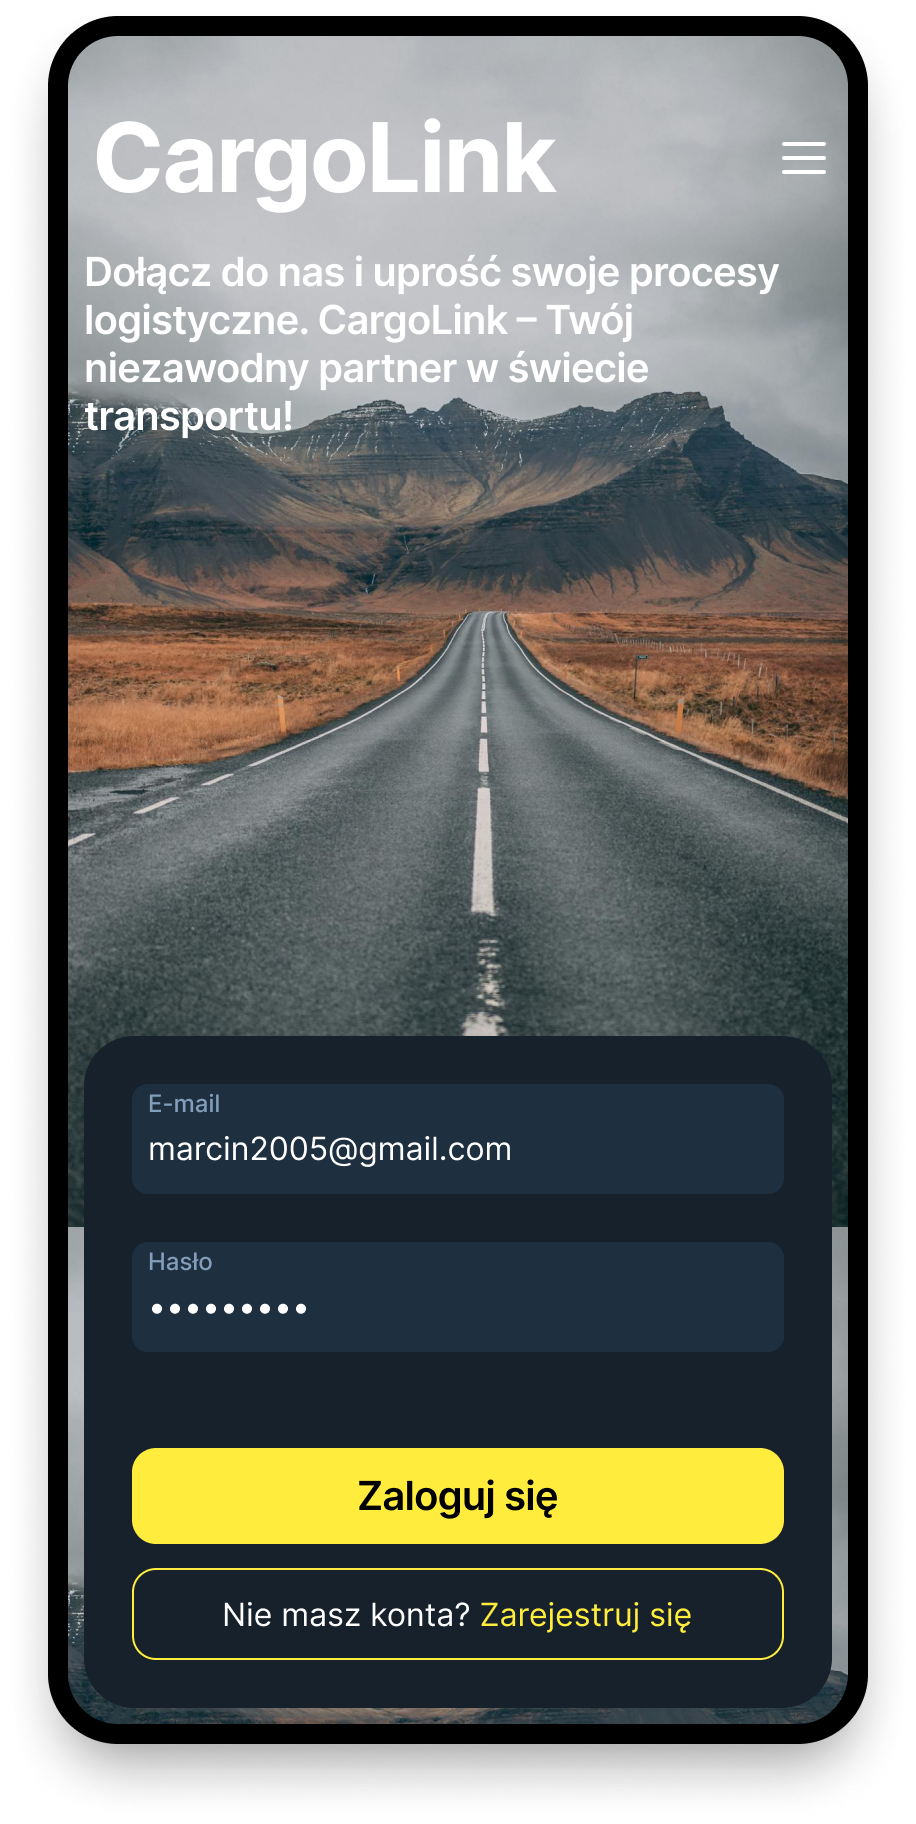
\includegraphics[width=0.3\textwidth]{rozdzial1/logowanie.png} &
  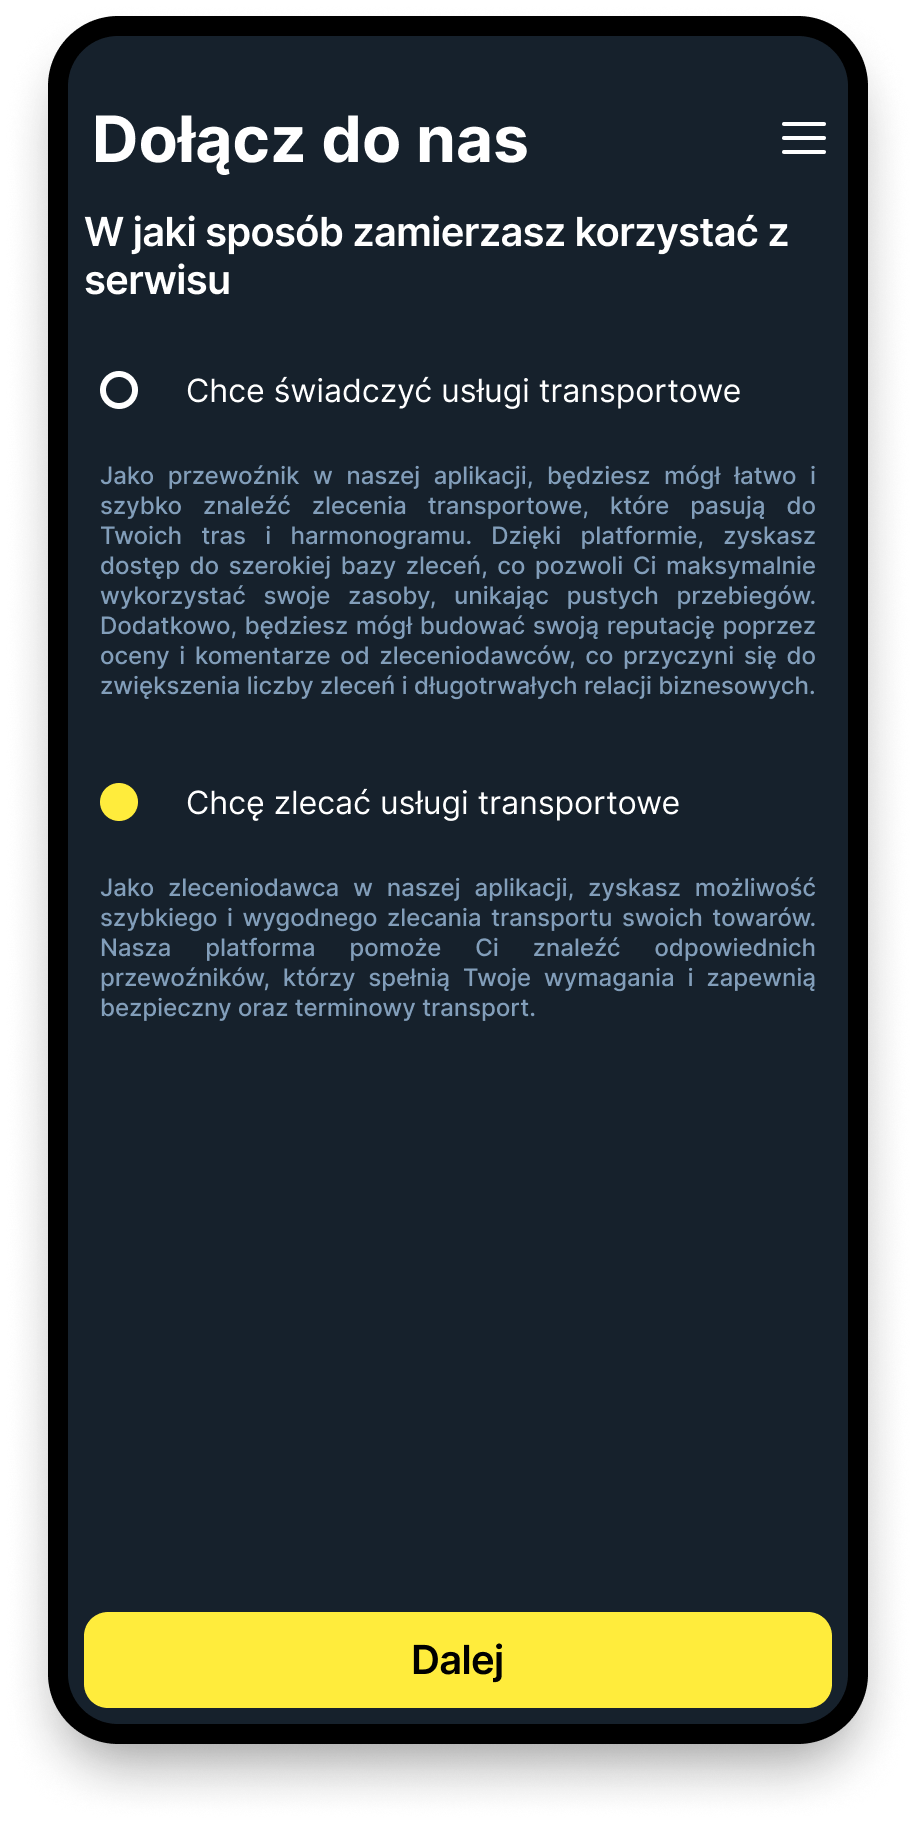
\includegraphics[width=0.3\textwidth]{rozdzial1/wybor_1.png} &
  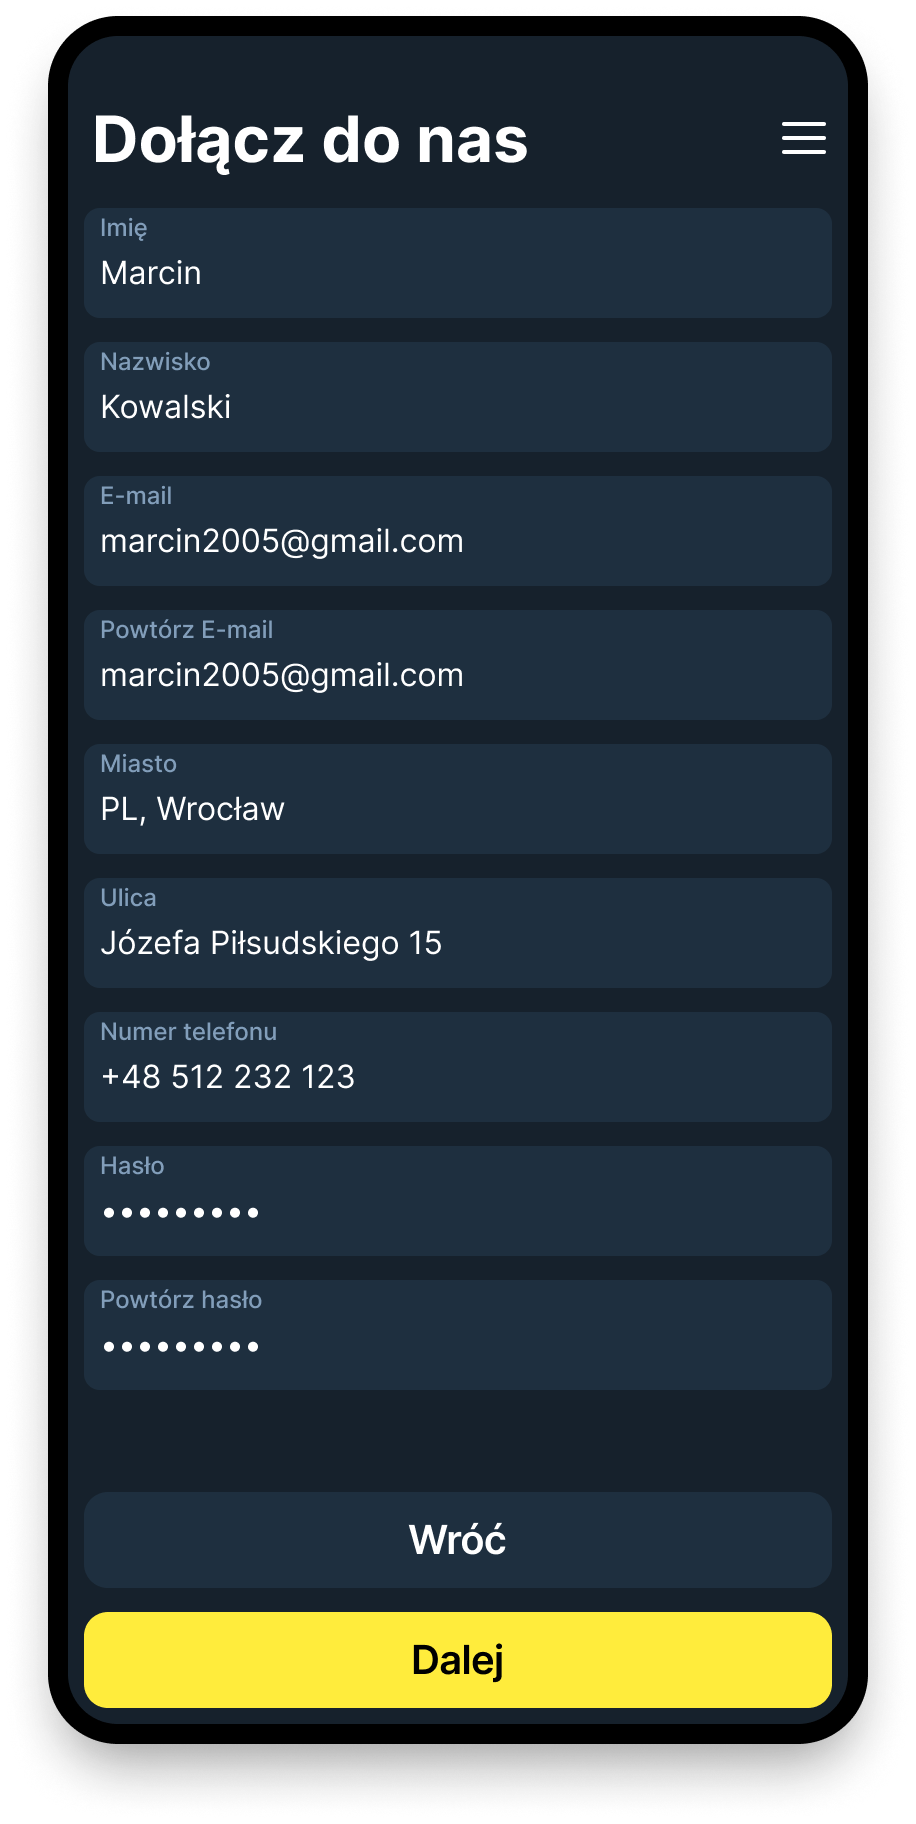
\includegraphics[width=0.3\textwidth]{rozdzial1/rejestracja.png}
  \end{tabular}
 \caption{Formularz rejestracji: a) Menu logowania, b) Wybór typu konta, c) Wprowadzenie danych do rejestracji}
 \label{fig:Formularz rejestracji - abc}
\end{figure}
\begin{figure}[H]
 \centering
  \begin{tabular}{@{}ccc@{}}
  d) & e)\\
  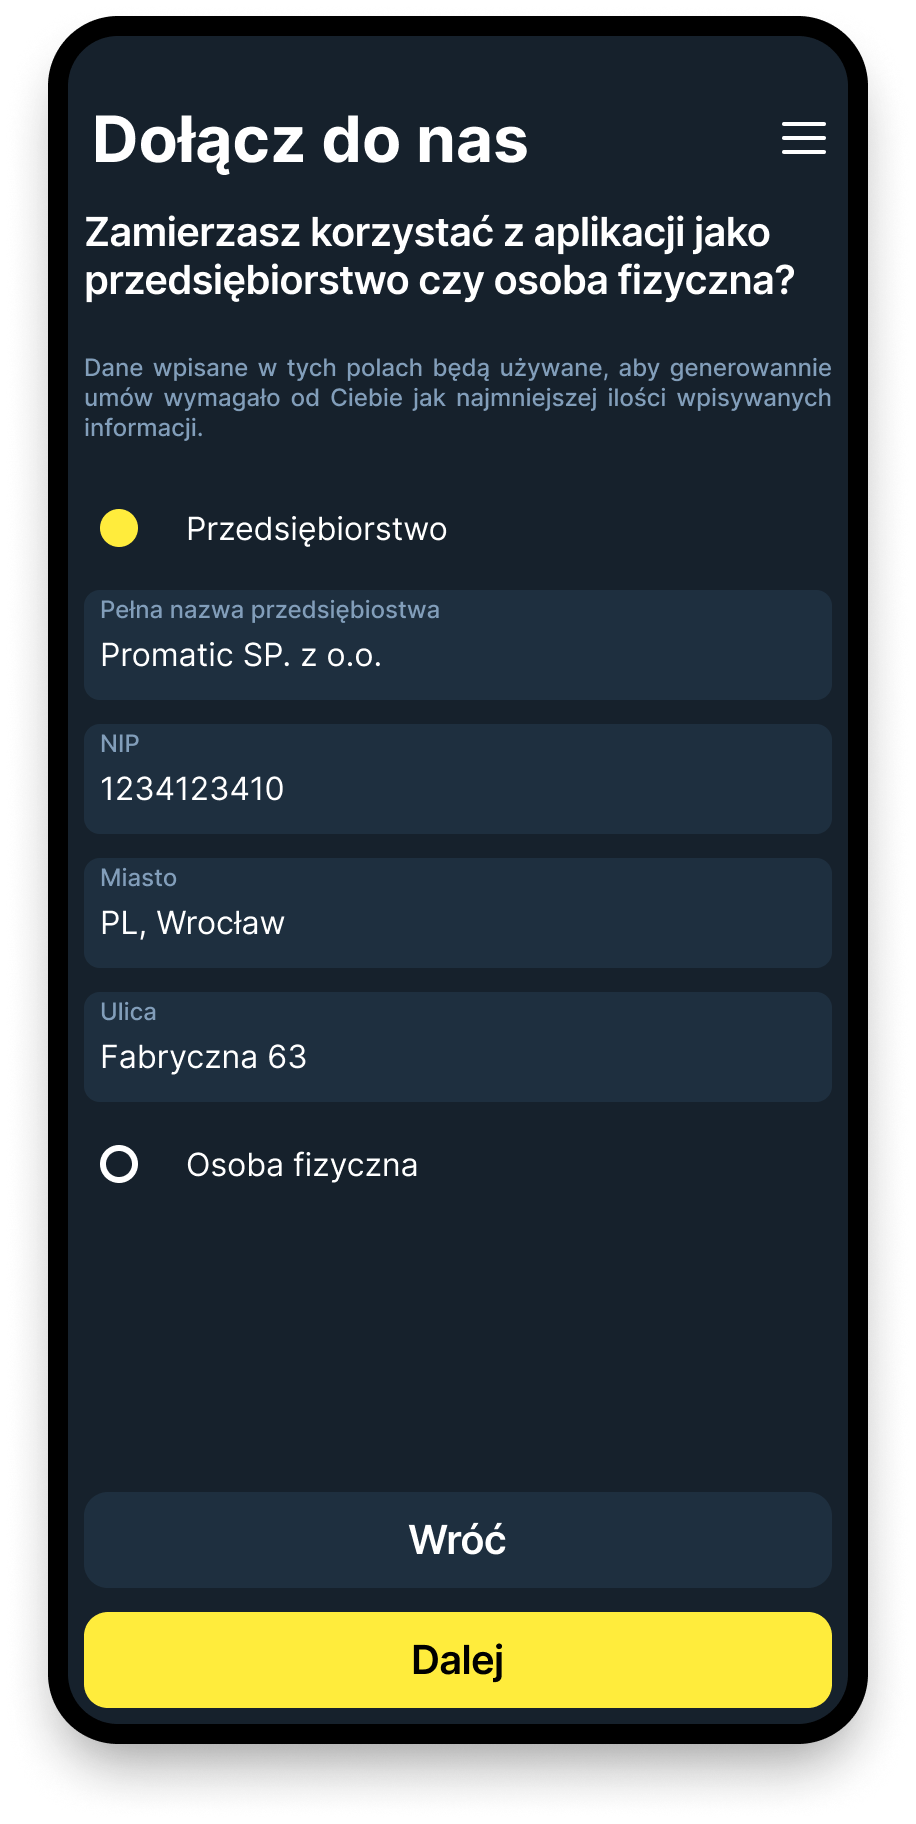
\includegraphics[width=0.3\textwidth]{rozdzial1/wybor_2.png} &
  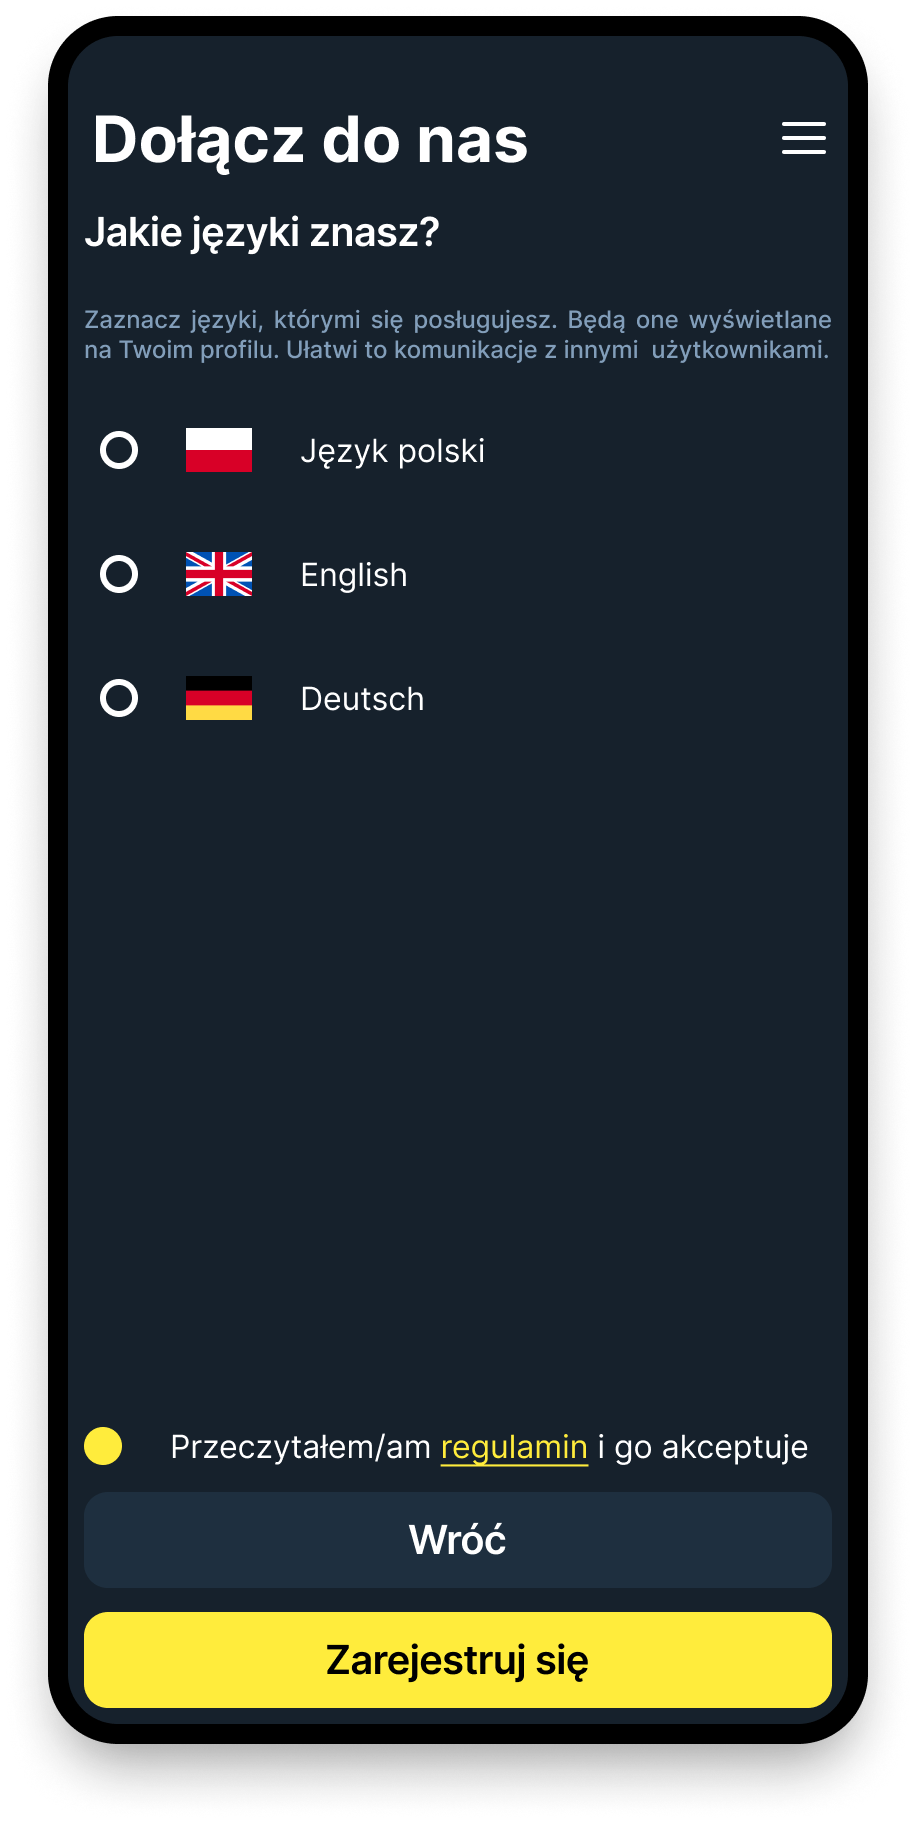
\includegraphics[width=0.3\textwidth]{rozdzial1/wybor_3.png} &
  \end{tabular}
 \caption{Formularz rejestracji: d) Wybór reprezentacji konta, e) Wybór języków, którymi użytkownik się posługuje, }
 \label{fig:Formularz rejestracji - de}
\end{figure}

\textbf{Logowanie} \\
Zdarzenie inicjujące: Wpisanie danych logowania oraz kliknięcie przycisku \texttt{Zaloguj się}. \\
Warunki początkowe: Użytkownik nie jest zalogowany. \\
Przebieg podstawowy realizacji przypadku użycia:
\begin{enumerate}
    \item Wpisanie danych, email oraz hasło:
    \item Kliknięcie przycisku \texttt{Zaloguj się}; (Rys. \ref{fig:Formularz rejestracji - abc}.a)
    \item System sprawdza w bazie danych czy istnieje już użytkownik o podanym emailu oraz czy wprowadzone hasło jest prawidłowe;
    \item Zalogowanie użytkownika;
    \item Przejście do wyszukiwarki ogłoszeń o planowanych trasach, bądź zleceń (w zależności od wybranego typu konta).
\end{enumerate}
Przebieg alternatywny realizacji przypadku użycia: W bazie danych nie znajduję się użytkownik o podanym emailu oraz haśle. System informuje o niepowodzeniu. \\
Warunki Końcowe: W zależności od typu konta, przenosi do odpowiedniego miejsca w serwisie.\\

\textbf{Zmiana wersji językowej} \\
Zdarzenie inicjujące: Kliknięcie w trzy poziome kreski w nagłówku, aby otworzyć menu (np. Rys. \ref{fig:Formularz rejestracji - abc}.a). \\
Warunki początkowe: Brak. \\
Przebieg podstawowy realizacji przypadku użycia:
\begin{enumerate}
    \item Kliknięcie w trzy poziome kreski w nagłówku, aby otworzyć menu (np. Rys. \ref{fig:Formularz rejestracji - abc}.a);
    \item Kliknięcie przycisku z ikoną globu (Rys. \ref{Rys. fig:Menu nawigacji po aplikacji - fg}.f);
    \item Wybranie jednego z trzech języków z menu (Rys. \ref{Rys. fig:Menu nawigacji po aplikacji - fg}.g);
    \item Zmienienie języka w jakim wyświetlana jest aplikacja;
\end{enumerate}
\begin{figure}[H]
	\centering
        \begin{tabular}{@{}ccc@{}}
            f) & g)\\
		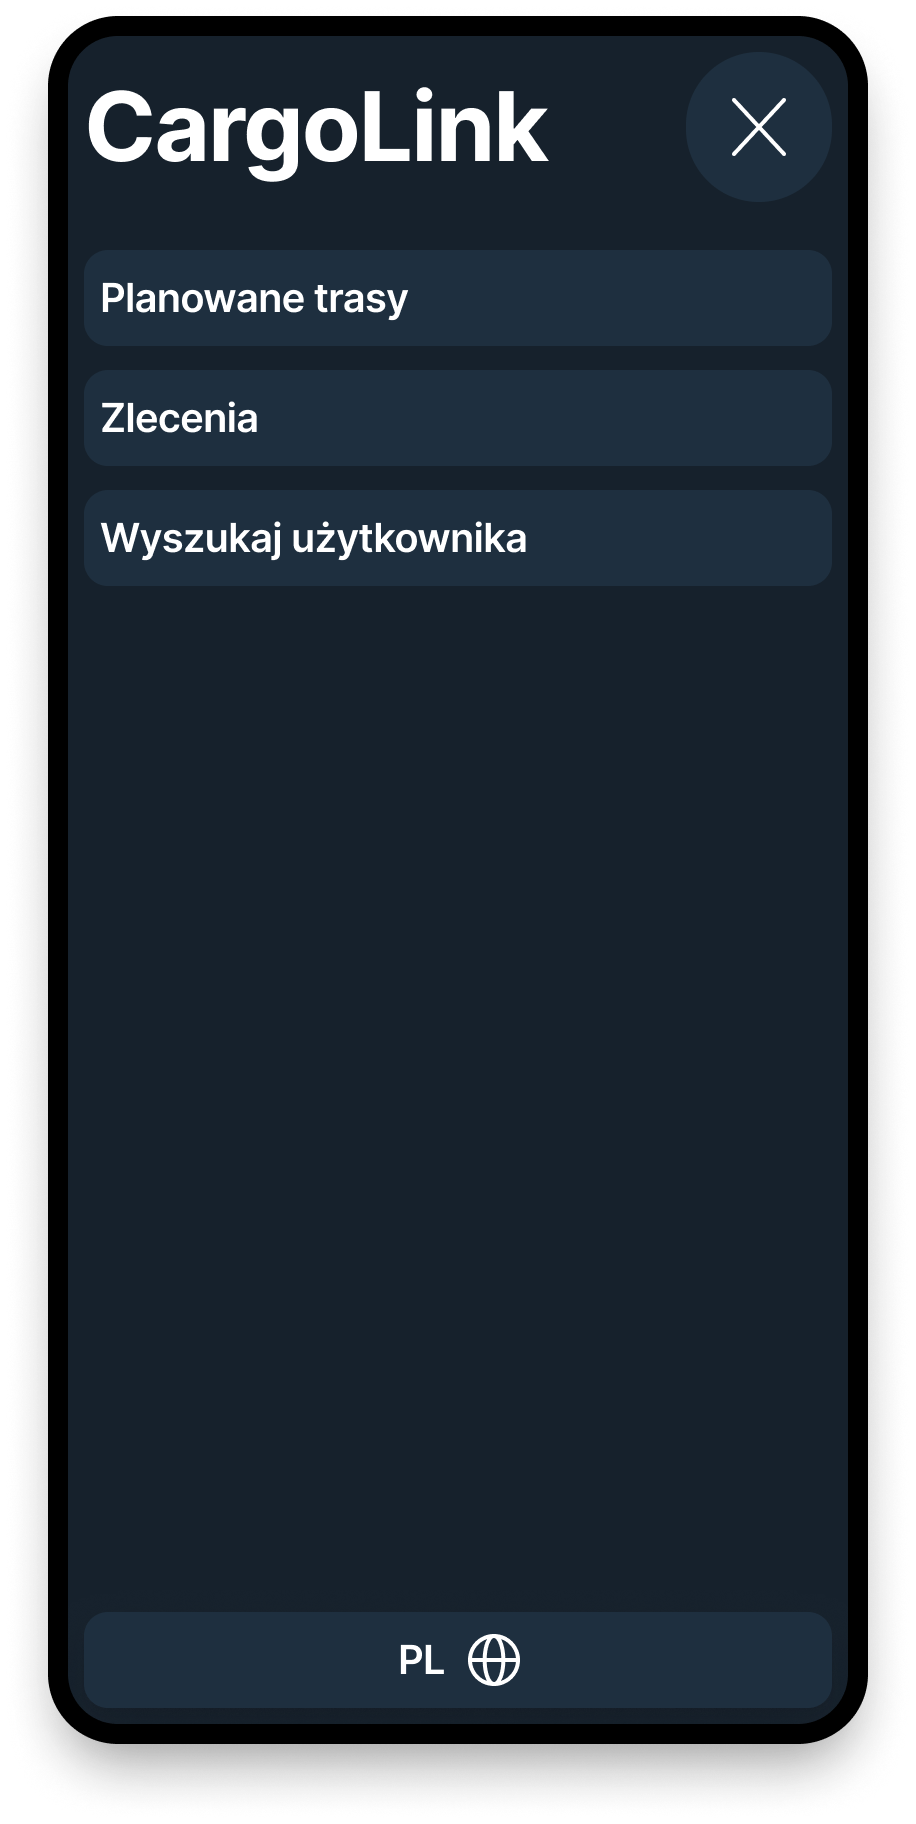
\includegraphics[width=0.3\linewidth]{rozdzial1/menu.png} &
		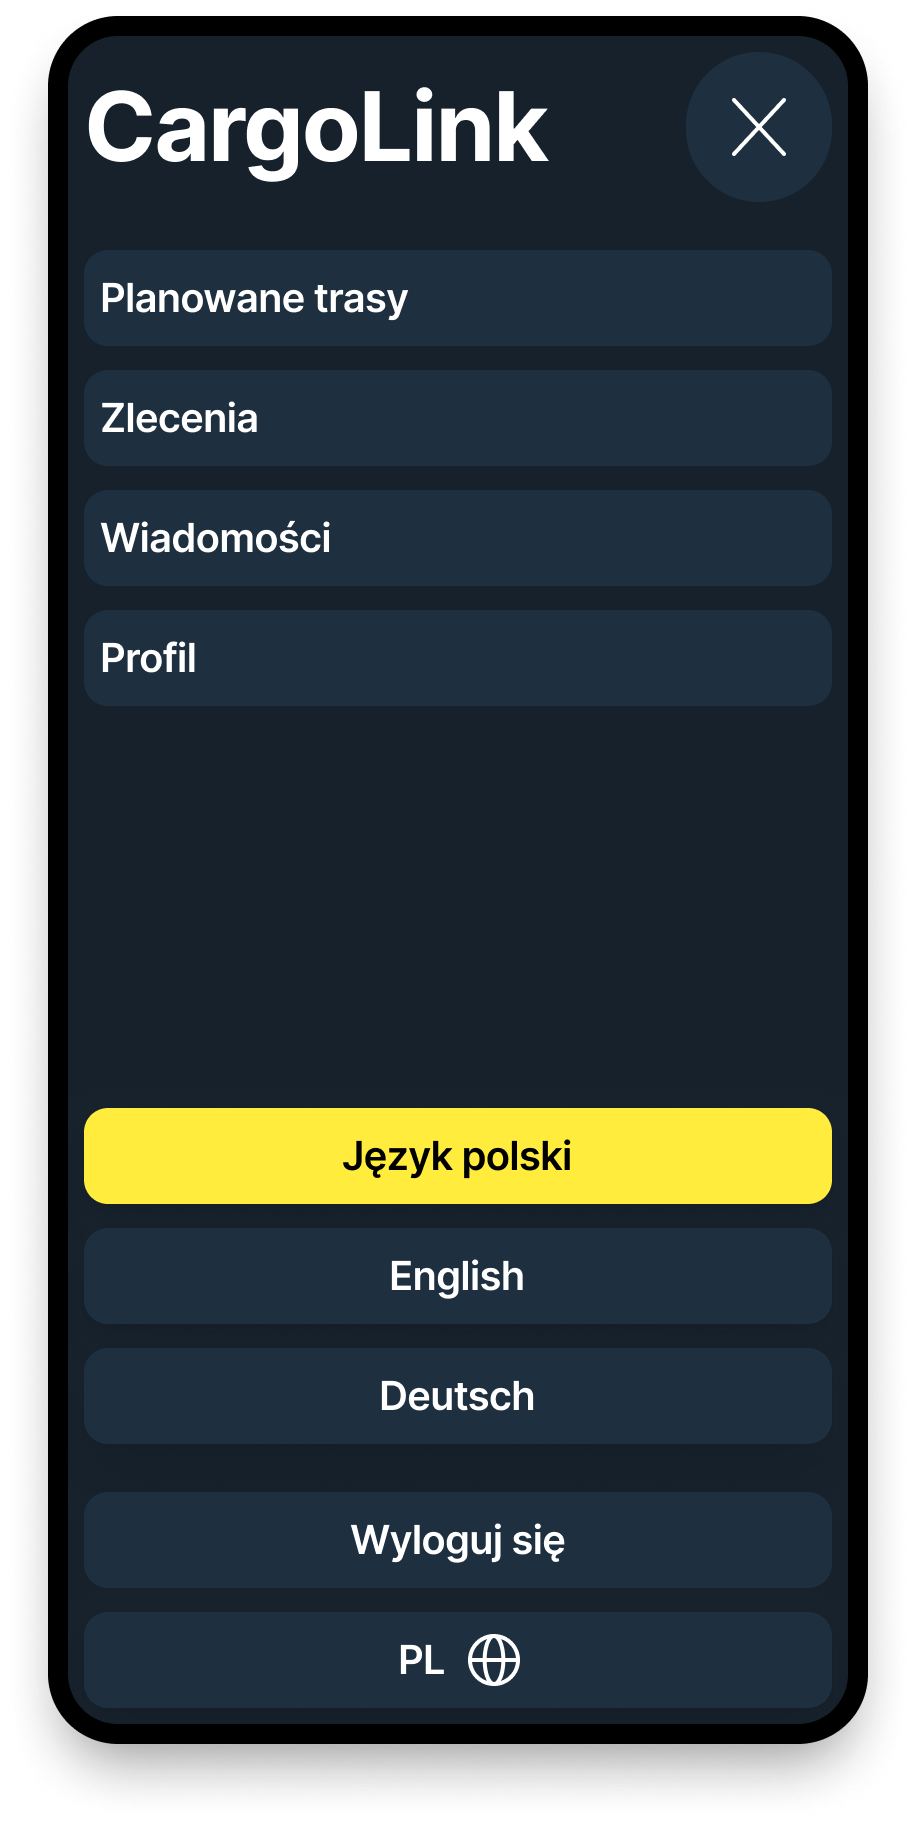
\includegraphics[width=0.3\linewidth]{rozdzial1/menu_język.png}
		\end{tabular}
	\caption{Menu nawigacji po aplikacji: f) Menu nawigacji, g) Menu nawigacji z klikniętym przyciskiem wyboru języka}
	\label{Rys. fig:Menu nawigacji po aplikacji - fg}
\end{figure}

\textbf{Wyszukiwanie użytkowników} \\
Zdarzenie inicjujące: Kliknięcie w trzy poziome kreski w nagłówku, aby otworzyć menu (np. Rys. \ref{fig:Formularz rejestracji - abc}.a). \\
Warunki początkowe: Brak. \\
Przebieg podstawowy realizacji przypadku użycia:
\begin{enumerate}
    \item Kliknięcie w trzy poziome kreski w nagłówku, aby otworzyć menu (np. Rys. \ref{fig:Formularz rejestracji - abc}.a);
    \item Kliknięcie przycisku \texttt{Wyszukaj użytkownika} (Rys. \ref{Rys. fig:Menu nawigacji po aplikacji - fg}.f);
    \item Wpisanie danych szukanego użytkownika, takich jak imię, nazwisko, e-mail lub typ konta (Rys. \ref{Rys. fig:Wyszukiwanie użytkownika});
    \item Kliknięcie przycisku \texttt{Szukaj} (Rys. \ref{Rys. fig:Wyszukiwanie użytkownika});
\end{enumerate}
Przebieg alternatywny realizacji przypadku użycia: W bazie danych nie znajduję się użytkownik spełniający wpisane wymagania. System informuje o niepowodzeniu. \\
Warunki Końcowe: Serwis zwraca wszystkie profile spełniające wpisane wymagania.\\
\begin{figure}[H]
	\centering
		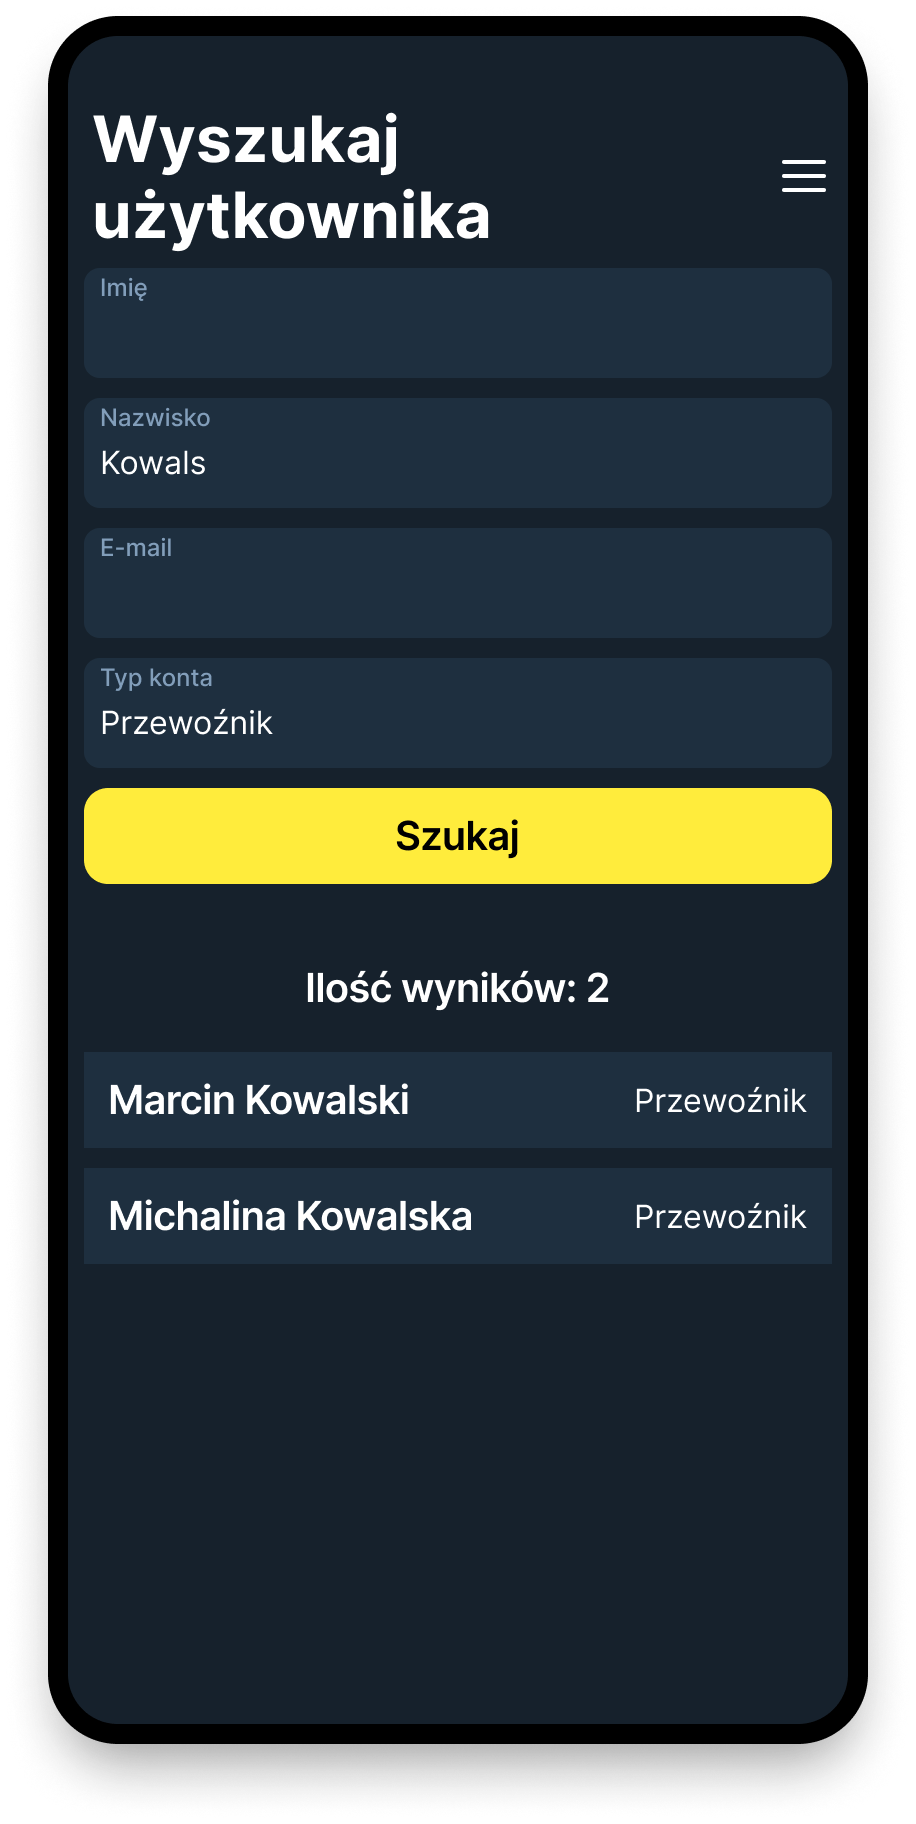
\includegraphics[width=0.3\linewidth]{rozdzial1/szukaj_uzytkownika.png}
	\caption{Wyszukiwanie użytkownika}
	\label{Rys. fig:Wyszukiwanie użytkownika}
\end{figure}
\label{Przeglądanie zleceń}

\textbf{Przeglądanie zleceń} \\
Zdarzenie inicjujące: Kliknięcie w trzy poziome kreski w nagłówku, aby otworzyć menu (np. Rys. \ref{fig:Formularz rejestracji - abc}.a). \\
Warunki początkowe: Brak. \\
Przebieg podstawowy realizacji przypadku użycia:
\begin{enumerate}
    \item Kliknięcie w trzy poziome kreski w nagłówku, aby otworzyć menu (np. Rys. \ref{fig:Formularz rejestracji - abc}.a);
    \item Kliknięcie przycisku \texttt{Zlecenia} (Rys. \ref{Rys. fig:Menu nawigacji po aplikacji - fg}.f);
\end{enumerate}
Przebieg alternatywny realizacji przypadku użycia: Brak. \\
Warunki Końcowe: Wyświetlenie przeglądarki zleceń. (Rys. \ref{Rys. fig:Przeglądarka zleceń i planowanych tras - hi}.h)
\begin{figure}[H]
	\centering
	\begin{tabular}{@{}ccc@{}}
            h) & i)\\
    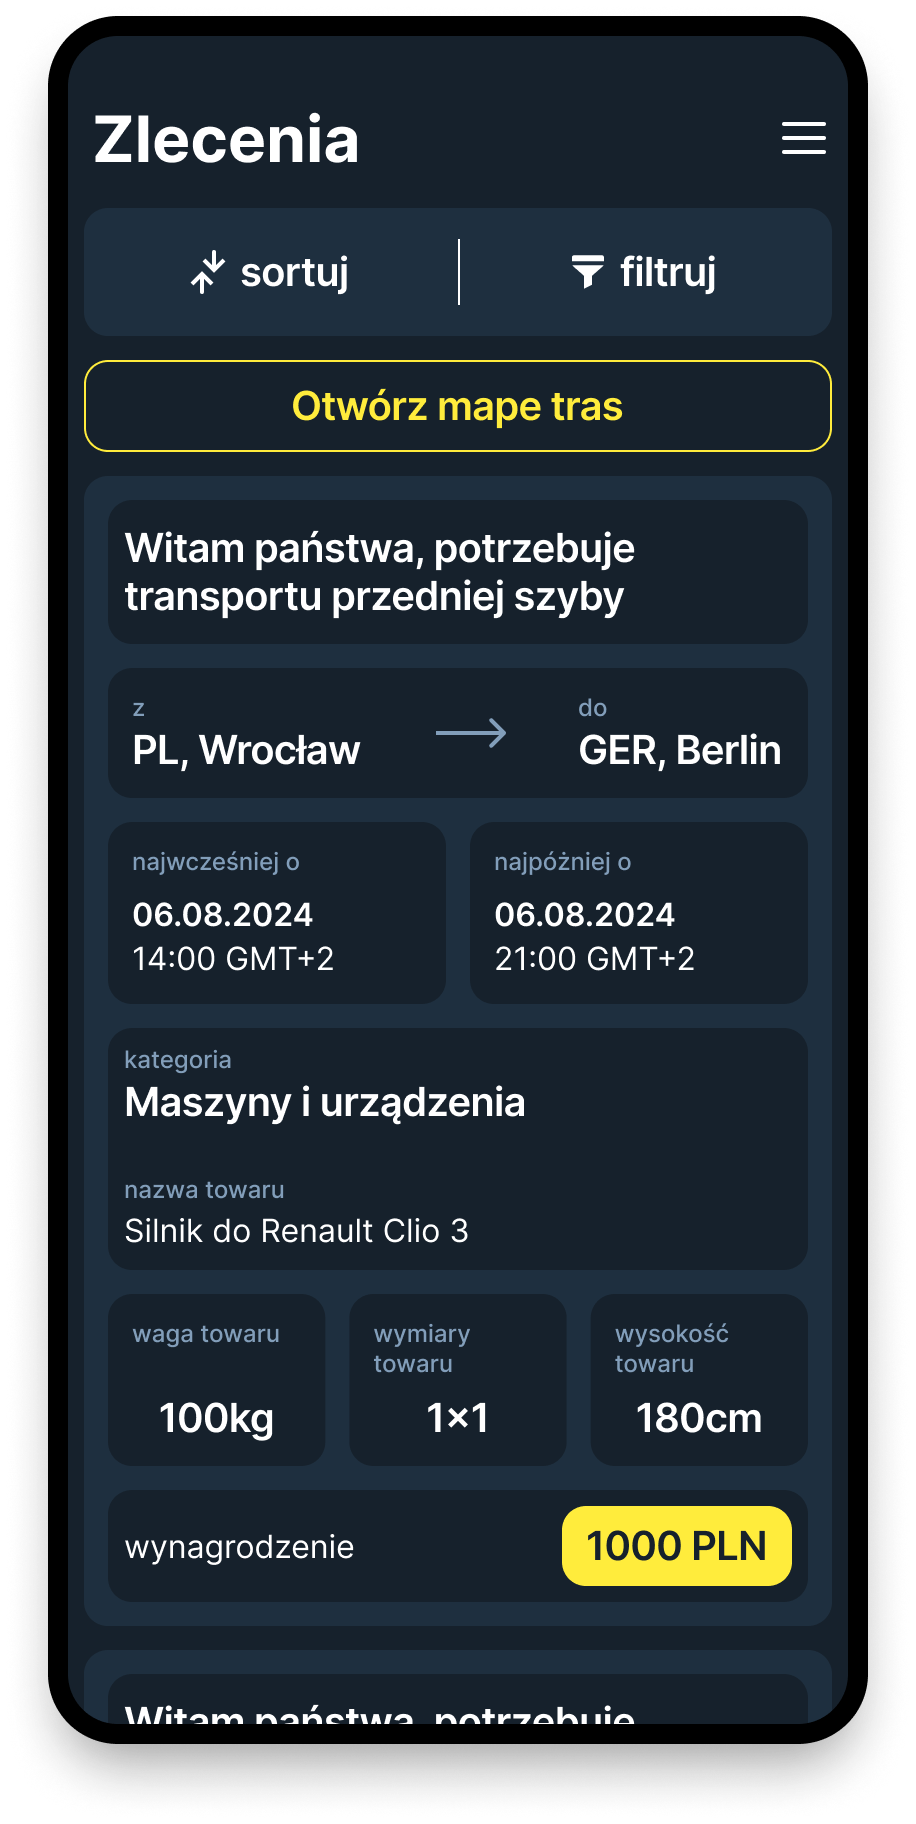
\includegraphics[width=0.3\linewidth]{rozdzial1/zlecenia.png} &
    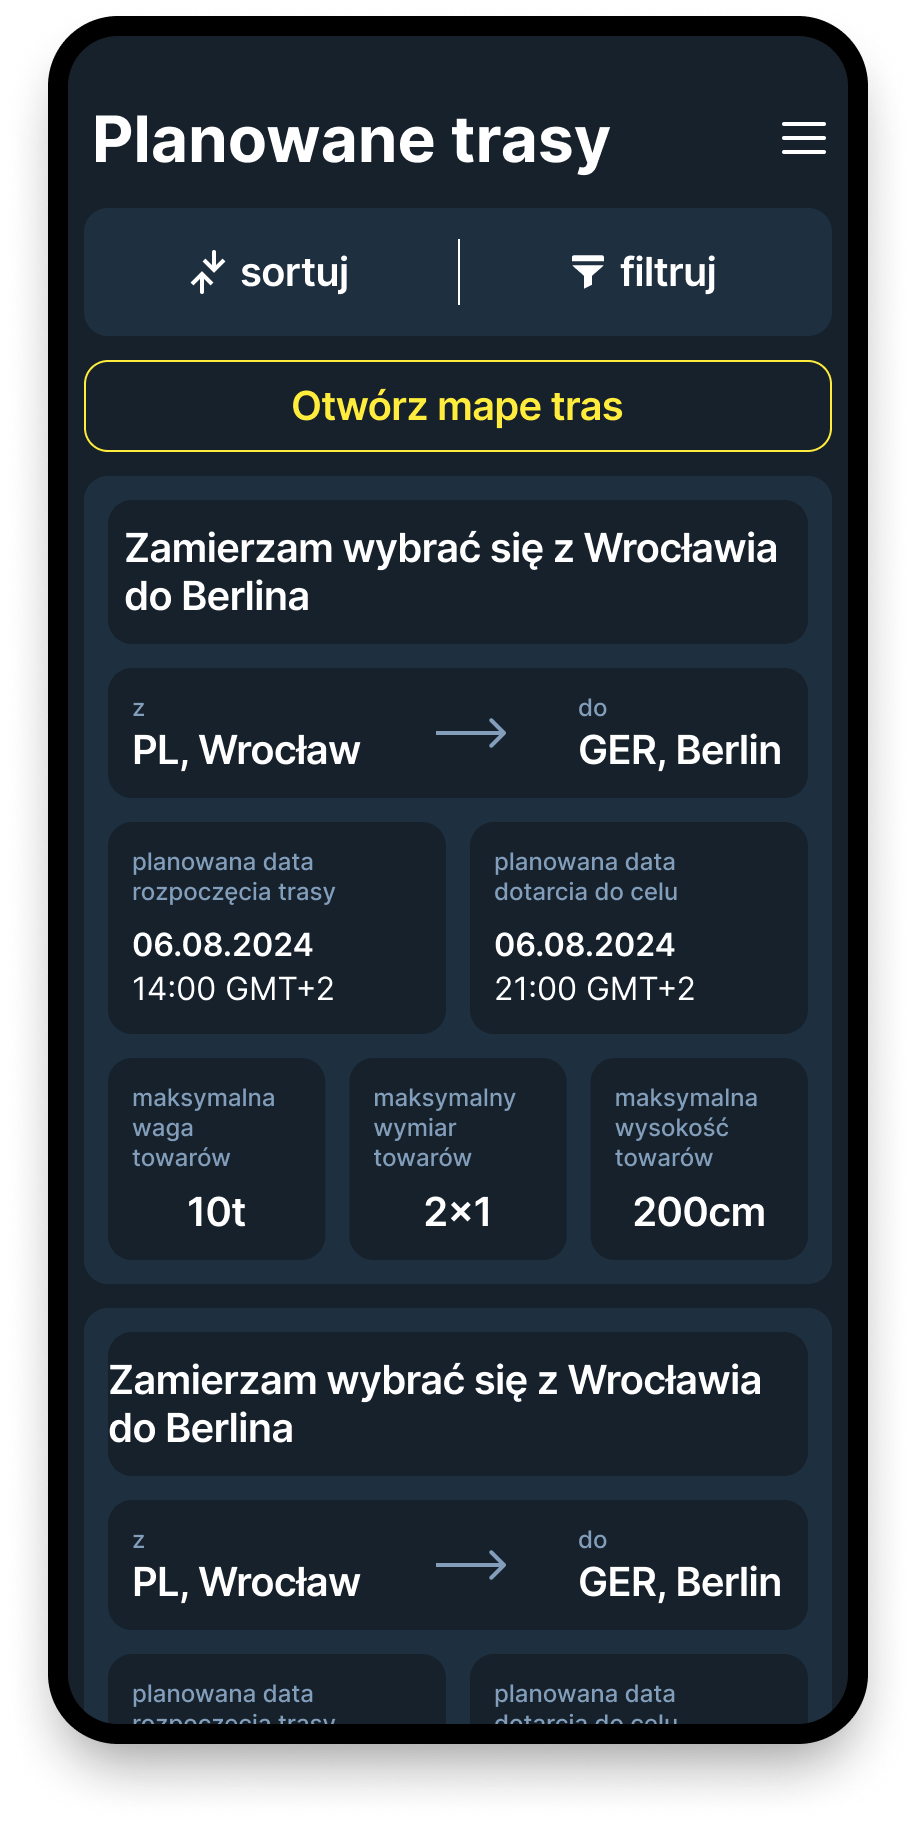
\includegraphics[width=0.3\linewidth]{rozdzial1/planowane_trasy.png}
    \end{tabular}
    \caption{Przeglądarka zleceń i planowanych tras: h) Przeglądarka zleceń, i) Przeglądarka ogłoszeń planowanych tras}
	\label{Rys. fig:Przeglądarka zleceń i planowanych tras - hi}
\end{figure}
\label{Przeglądanie ogłoszeń planowanych tras}

\textbf{Przeglądanie ogłoszeń planowanych tras} \\
Zdarzenie inicjujące: Kliknięcie w trzy poziome kreski w nagłówku, aby otworzyć menu (np. Rys. \ref{fig:Formularz rejestracji - abc}.a). \\
Warunki początkowe: Brak. \\
Przebieg podstawowy realizacji przypadku użycia:
\begin{enumerate}
    \item Kliknięcie w trzy poziome kreski w nagłówku, aby otworzyć menu (np. Rys. \ref{fig:Formularz rejestracji - abc}.a);
    \item Kliknięcie przycisku \texttt{Planowane trasy} (Rys. \ref{Rys. fig:Menu nawigacji po aplikacji - fg}.f);
\end{enumerate}
Przebieg alternatywny realizacji przypadku użycia: Brak. \\
Warunki Końcowe: Wyświetlenie przeglądarki ogłoszeń o planowanych trasach. (Rys. \ref{Rys. fig:Przeglądarka zleceń i planowanych tras - hi}.i)\\

\textbf{Wyświetlenie ogłoszenia} \\
Zdarzenie inicjujące: Kliknięcie w dowolne ogłoszenie (Rys. \ref{Rys. fig:Przeglądarka zleceń i planowanych tras - hi}.h lub \ref{Rys. fig:Przeglądarka zleceń i planowanych tras - hi}.i). \\
Warunki początkowe: Brak. \\
Przebieg podstawowy realizacji przypadku użycia:
\begin{enumerate}
    \item Wykonanie przypadku użycia \ref{Przeglądanie zleceń} lub \ref{Przeglądanie ogłoszeń planowanych tras}
    \item Kliknięcie w dowolne ogłoszenie (Rys. \ref{Przeglądanie zleceń});
\end{enumerate}
Przebieg alternatywny realizacji przypadku użycia: Brak. \\
Warunki Końcowe: Wyświetlenie klikniętego ogłoszenia. (Rys. \ref{Rys. fig:Wyświetlenie ogłoszenia - jk}.j lub \ref{Rys. fig:Wyświetlenie ogłoszenia - jk}.k)
\begin{figure}[H]
	\centering
	\begin{tabular}{@{}ccc@{}}
            j) & k)\\
    \vtop{\null\hbox{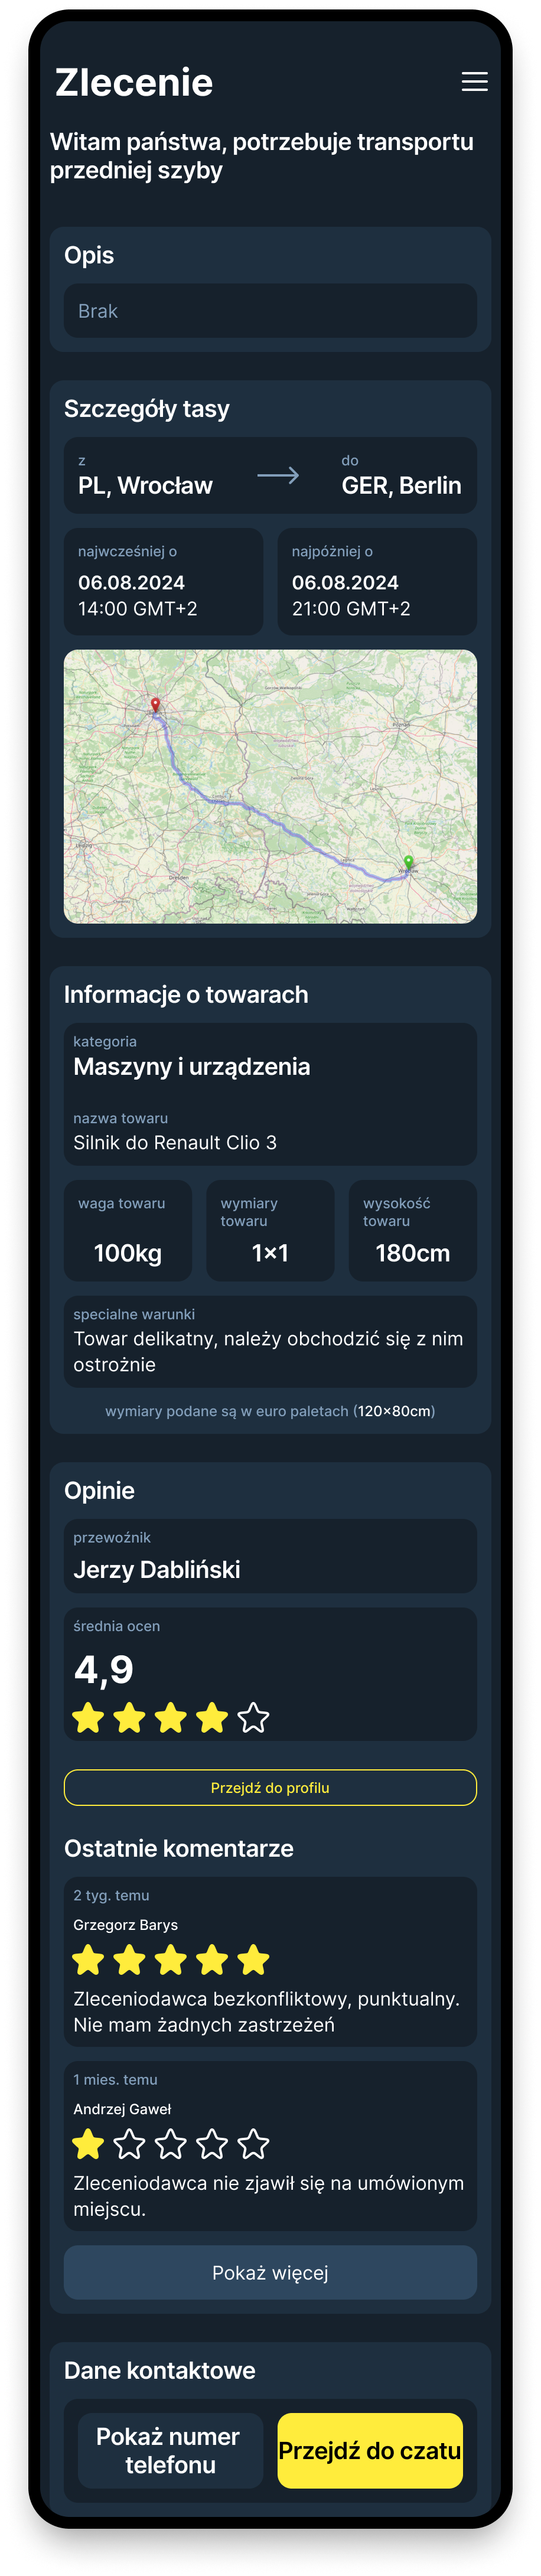
\includegraphics[width=0.25\linewidth]{rozdzial1/ogloszenie_zlecenie.png}}} &
    \vtop{\null\hbox{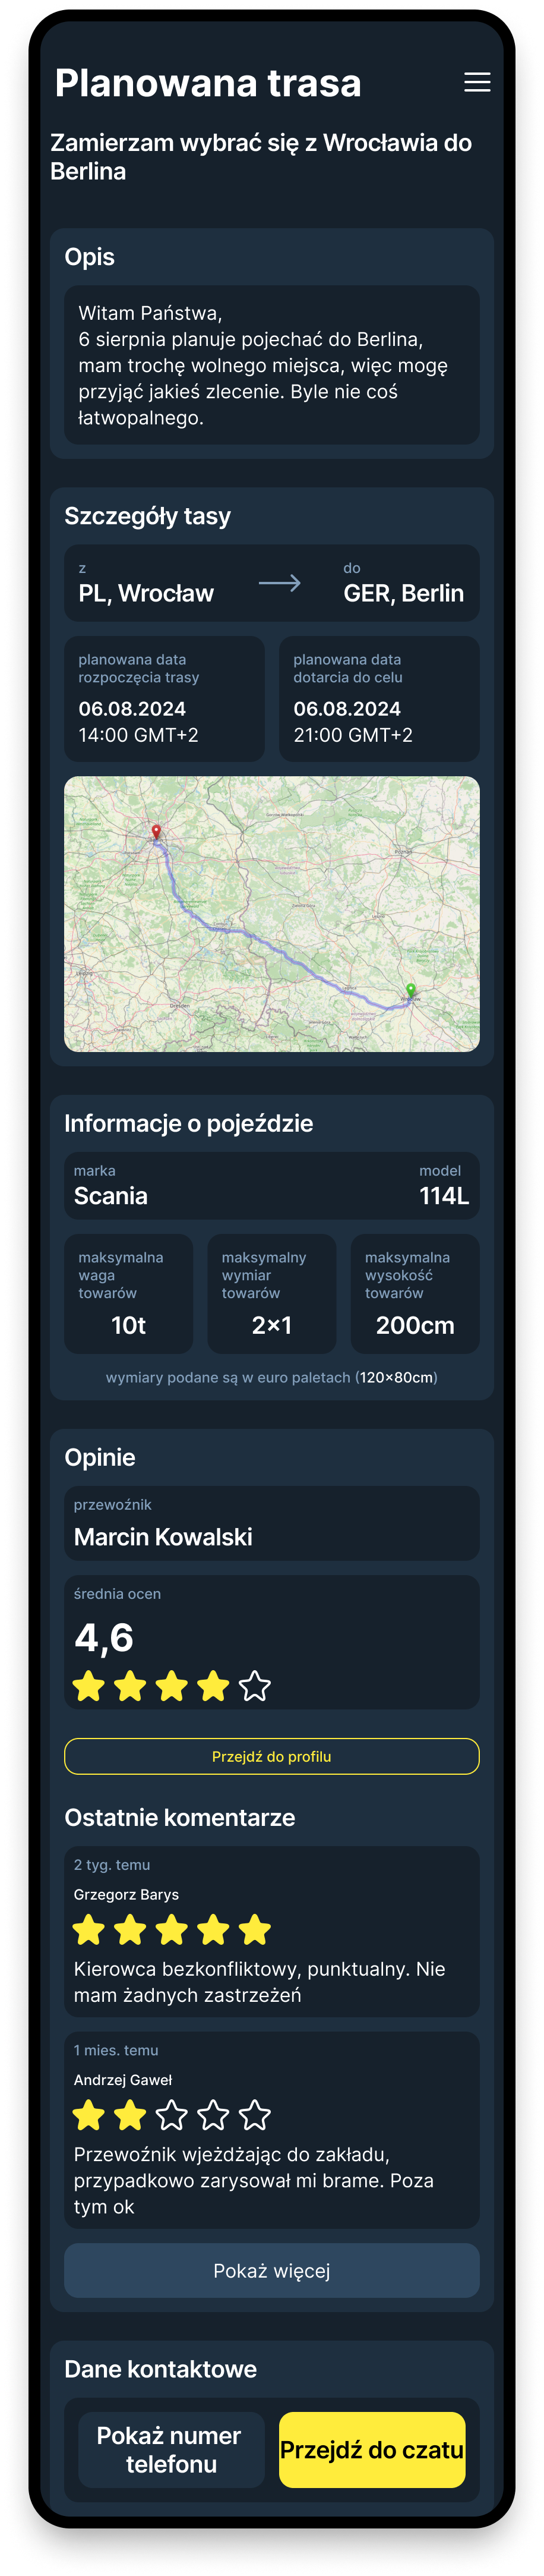
\includegraphics[width=0.25\linewidth]{rozdzial1/ogloszenie_planowana_trasa.png}}}
    \end{tabular}
    \caption{Wyświetlenie ogłoszenia: j) Ogłoszenie zlecenia, k) Ogłoszenie o planowanej trasie}
	\label{Rys. fig:Wyświetlenie ogłoszenia - jk}
\end{figure}

\textbf{Wyświetlenie mapy ze wszystkimi trasami} \\
Zdarzenie inicjujące: Kliknięcie w przycisk \texttt{Otwórz mape tras} (Rys. \ref{Przeglądanie zleceń} lub \ref{Przeglądanie ogłoszeń planowanych tras}). \\
Warunki początkowe: Brak. \\
Przebieg podstawowy realizacji przypadku użycia:
\begin{enumerate}
    \item Wykonanie przypadku użycia \ref{Przeglądanie zleceń} lub \ref{Przeglądanie ogłoszeń planowanych tras}
    \item Kliknięcie w przycisk \texttt{Otwórz mape tras} (Rys. \ref{Przeglądanie zleceń} lub \ref{Przeglądanie ogłoszeń planowanych tras}).    
\end{enumerate}
Przebieg alternatywny realizacji przypadku użycia: Brak. \\
Warunki Końcowe: Użytkownikowi ukazuję się mapa z zaznaczonymi trasami wszystkich ogłoszeń w bazie danych (Rys. \ref{Rys. fig:Mapa ze wszystkimi trasami}).\\
\begin{figure}[H]
	\centering
		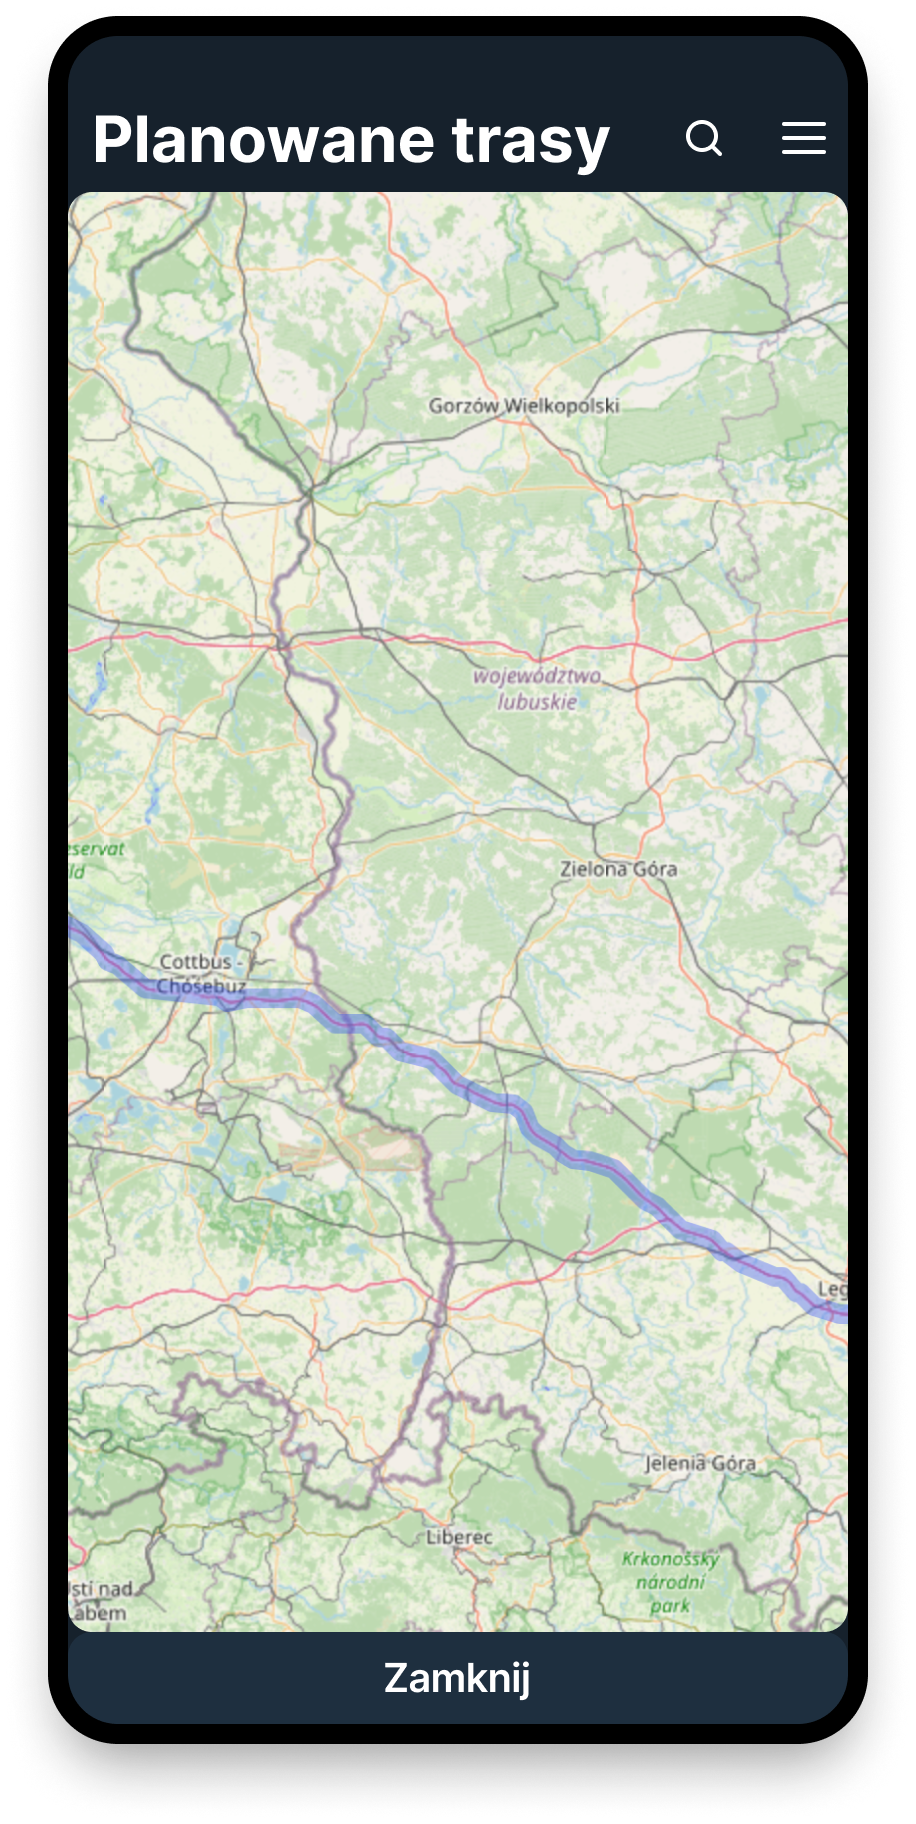
\includegraphics[width=0.3\linewidth]{rozdzial1/mapa.png}
	\caption{Mapa ze wszystkimi trasami}
	\label{Rys. fig:Mapa ze wszystkimi trasami}
\end{figure}